\bookchapter{Kapitel 49: Die Entwicklungsumgebung einrichten – Android Studio und das erste Projekt}

\chapterintro{Werkzeug muss sitzen, bevor die Arbeit beginnt. In diesem Kapitel bauen wir die “Küche” auf: Android Studio installieren, den Emulator zum Laufen bringen, das erste Android-Projekt deines Lebens anlegen und die Projektstruktur auseinandernehmen, bis alles klar ist. Wenn die Umgebung steht, siehst du zum ersten Mal, wie dein eigener Code zu einem tippbaren Button wird – diesen Moment merken sich viele ein Leben lang.}

\booksection{Android Studio installieren}

Android Studio ist die offizielle integrierte Entwicklungsumgebung (IDE) von Google – kostenlos und als Komplettpaket: Code schreiben, Vorschau der Oberfläche ansehen, debuggen, Pakete bauen, alles darin. Die Installation hat vier Schritte:

\begin{enumerate}
  \item Öffne die offizielle Website developer.android.com/studio und lade die neueste stabile Version herunter (im August 2026 die Version nach Narwhal; für Windows/Mac/Linux verfügbar);
  \item Starte das Installationspaket und klicke dich mit "Weiter" durch – der Assistent bringt Android SDK und Emulator-Komponenten automatisch mit;
  \item Beim ersten Start lädst du nach Aufforderung die SDK-Komponenten herunter (die Standardauswahl passt; das kann ein paar Minuten und einige GB Speicher brauchen);
  \item Danach siehst du die Willkommensseite – Glückwunsch, die "Küche" steht.
\end{enumerate}

\begin{tcbwarn}{Achtung: Die Hardware-Anforderungen im Blick behalten}
Android Studio ist ein echter “Speicherfresser”: plane mindestens 16 GB RAM ein (8 GB gehen auch, aber der Emulator ruckelt dann schnell), reserviere über 20 GB Speicherplatz und sorge für eine CPU mit Virtualisierung (VT-x/AMD-V im BIOS aktivieren). Wenn dein Rechner wirklich alt ist, nutze statt des Emulators das Debuggen auf dem echten Gerät (Abschnitt 4 dieses Kapitels) – das läuft oft sogar flüssiger.

\end{tcbwarn}

\booksection{Dein erstes Projekt anlegen}

Klicke auf der Willkommensseite auf New Project, wähle die Vorlage Empty Activity (die sauberste Einsteiger-Vorlage) und fülle drei Dinge aus:

\begin{center}
\begin{tabularx}{\linewidth}{|X|X|X|}
\hline
\textbf{Einstellung} & \textbf{Was eintragen?} & \textbf{Erklärung} \tabularnewline
\hline
Name & My First App & Der Name der App, erscheint auf dem Startbildschirm des Telefons \tabularnewline
Package name & com.example.myfirstapp & Weltweit eindeutige Kennung, üblich ist der umgedrehte Domainname – nimm zunächst den Standard \tabularnewline
Minimum SDK & API 26(Android 8.0) & Mindestens unterstützte Version, deckt über 95 \% der Geräte ab \tabularnewline
\hline
\end{tabularx}
\end{center}

\begin{center}\small\color{gray}Die drei Angaben beim Anlegen eines Projekts\end{center}

Nach einem Klick auf Finish lädt Android Studio per Gradle automatisch die Abhängigkeiten und baut das Projekt (beim ersten Mal dauert es ein paar Minuten, danach geht es jedes Mal viel schneller). Wenn der Build fertig ist, hast du eine lauffähige App – auch wenn sie vorerst nur “Hello Android!” anzeigt.

\begin{tcbinfo}{Tipp: Was es mit dem Paketnamen auf sich hat}
Der Paketname (package name) ist wie der “Personalausweis” der App – weltweit einmalig und nach der Veröffentlichung nicht mehr änderbar. Für private Übungen reicht com.example.xxx; für ein echtes Produkt nimm den umgedrehten eigenen Domainnamen (z. B. com.deinname.appname). Veröffentliche nichts unter com.example – der Store lehnt das ab.

\end{tcbinfo}

\booksection{Ans Laufen bringen: Emulator und echtes Gerät}

Der Code ist geschrieben – jetzt braucht er ein “Telefon” zum Laufen. Du hast zwei Möglichkeiten:

\booksubsection{Der Emulator}

Der Emulator virtualisiert ein Android-Telefon im Computer. Öffne in Android Studio den Device Manager Create Device, wähle ein Gerät (empfohlen: die Pixel-Serie) wähle ein Systemabbild (mit Google APIs) lade es herunter starte. Dann klickst du auf das grüne Dreieck Run in der Symbolleiste, und nach ein paar Sekunden erscheint deine App auf dem Bildschirm des “Telefons”.

\booksubsection{Debuggen auf dem echten Gerät (noch empfehlenswerter)}

Ein echtes Gerät ist und bleibt die realistischste Testumgebung – Wischgefühl, echtes Netz, echte Sensoren: Der Emulator kommt da nicht mit. Das Debuggen auf einem Android-Gerät ist ganz einfach:

\begin{enumerate}
  \item Öffne auf dem Telefon [Einstellungen] [Über das Telefon] und tippe 7-mal hintereinander auf "Buildnummer", um die "Entwickleroptionen" freizuschalten;
  \item Aktiviere in den [Entwickleroptionen] USB-Debugging;
  \item Verbinde das Telefon per Datenkabel mit dem Computer und tippe im Pop-up des Telefons "USB-Debugging erlauben" an;
  \item Zurück in Android Studio erscheint dein Telefon in der Geräte-Dropdownliste der Symbolleiste – klicke auf Run.
\end{enumerate}

\textbf{Stolperfalle: USB-Debugging nicht dauerhaft aktiviert lassen}\par

USB-Debugging ist wie eine “Hintertür” für den Computer. Wenn du in der Öffentlichkeit lädst oder dich mit nicht vertrauenswürdigen Rechnern verbindest, schalte USB-Debugging unbedingt aus, damit niemand über diese Tür deine Daten auslesen kann. Mach es nach der Entwicklung immer wieder aus – das wird zur Gewohnheit.

\booksection{Die Projektstruktur zerlegt: wofür jede Datei gut ist}

Beim ersten Öffnen des Projekts kann dich der Dateibaum links schwindelig machen. Keine Panik – im Alltag verbringst du 90 \% deiner Zeit nur mit den folgenden paar Dateien:

\begin{center}
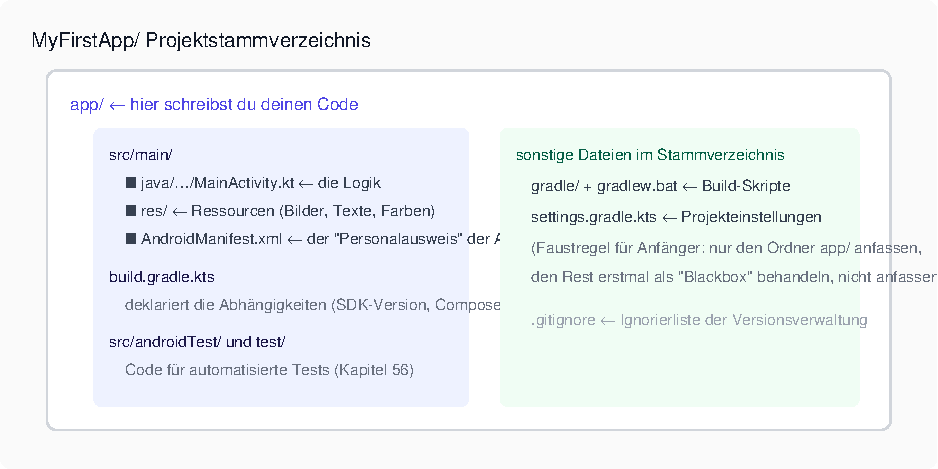
\includegraphics[width=0.92\linewidth]{figures/fig-di-si-shi-jiu-zhang-1}
\\[2pt]\small Abbildung 2: Die Projektstruktur, die Einsteiger kennen müssen (Merkregel: nur den Ordner app/ anfassen)
\end{center}

\begin{itemize}
  \item MainActivity.kt: das "Eingangstor" der App. Tippt der Nutzer auf das Symbol, wird es als erstes geweckt. In der heutigen Vorlage zeigt es "Hello Android!" an.
  \item AndroidManifest.xml: das "Melderegister" der App – hier steht, wie die App heißt, welches Symbol sie hat, welche Seiten es gibt und welche Berechtigungen sie braucht (Kamera, Standort usw.).
  \item res/-Ordner: das Ressourcenlager – hier liegen Bilder, Symbole, Texte, Farben. Texte in Ressourcendateien statt fest im Code zu hinterlegen, ist gute Android-Praxis (Sprach- und Themenwechsel werden so zum Kinderspiel).
  \item build.gradle.kts: das Baurezept – legt die unterstützte Mindestversion fest und welche Bibliotheken eingebunden sind (z. B. Compose).
\end{itemize}

\booksection{Erste Gehversuche: “Hello” durch deinen Namen ersetzen}

Öffne MainActivity.kt und schau dir den von der Compose-Vorlage erzeugten Code an. Finde die Zeile Text(“Hello Android!”) und ersetze den Text in den Anführungszeichen durch deinen Namen, z. B. Text(“Hallo, Max Mustermann! Das ist meine erste App”), und drücke Strg+R (auf dem Mac Cmd+R), um neu zu starten. Ein paar Sekunden später zeigt der Emulator deinen Namen.

\begin{lstlisting}[language=Kotlin]
setContent {
    MyFirstAppTheme {
        Surface(modifier = Modifier.fillMaxSize()) {
            // v hier deinen eigenen Text einsetzen
            Text("Hallo Max! Das ist meine erste App")
        }
    }
}
\end{lstlisting}

Glückwunsch – du hast soeben einen vollständigen Zyklus “Code ändern kompilieren installieren ausführen” hinter dich gebracht. Dieser Zyklus ist der Entwickleralltag der kommenden Tage. Mach gleich weiter: Ändere noch etwas anderes – vergrößere die Schrift, wechsle die Farbe. Im nächsten Kapitel lernst du, woher diese “Magie” kommt.

\booksection{Erste Hilfe bei häufigen Fehlermeldungen: die “Notaufnahme” für die ersten zwei Wochen}

Beim Aufsetzen der Umgebung und beim ersten Build wirst du mit hoher Wahrscheinlichkeit auf die folgenden drei Fehler stoßen. Keine Panik – für alle gibt es ein Gegenmittel:

\begin{center}
\begin{tabularx}{\linewidth}{|X|X|X|}
\hline
\textbf{Fehlerbild} & \textbf{Häufige Ursache} & \textbf{Gegenmittel} \tabularnewline
\hline
Gradle sync failed / Abhängigkeiten laden langsam & Der Zugriff auf die Repositorien über das Netz hakt & Für Gradle einen schnellen Maven-Spiegel einrichten (z. B. Alibaba Cloud oder Tencent Cloud) – suche online nach "gradle china mirror" und richte es nach der Anleitung ein \tabularnewline
SDK-Komponenten fehlen & Der SDK-Download wurde bei der Installation übersprungen & Unter Settings SDK Manager die fehlenden Plattformen und Tools nachinstallieren \tabularnewline
Emulator startet nicht / schwarzer Bildschirm & Virtualisierung nicht aktiviert, Abbild beschädigt & Im BIOS VT-x/AMD-V einschalten; den Emulator löschen und neu anlegen; oder gleich das echte Gerät zum Debuggen nehmen \tabularnewline
\hline
\end{tabularx}
\end{center}

\begin{center}\small\color{gray}Erste-Hilfe-Tabelle für Umgebungsfehler bei Einsteigern\end{center}

\begin{tcbinfo}{Tipp: Wie man Fehlermeldungen richtig sucht}
Die erste Zeile einer Fehlermeldung ist am wertvollsten – kopiere sie wortwörtlich in die Suchmaschine und ergänze das Stichwort “android studio”. Suche nicht nach vagen Fragen wie “Ich bringe meine Umgebung nicht zum Laufen”, sondern nach konkreten Fehlern wie “Gradle sync failed: Could not resolve com.android.tools.build”. Präzise Fragen bringen präzise Antworten.

\end{tcbinfo}

\begin{tcbpractice}{Selbst ausprobieren: Deine "Entwickler-Ritual"-Liste abhaken}
(1) Android Studio installieren und den Emulator zum Laufen bringen; (2) die eigene App einmal auf dem echten Gerät laufen lassen und einen Screenshot als Erinnerung machen; (3) den Hello-Text in deinen Namen ändern; (4) das Projekt zippen und archivieren. Nach diesen vier Schritten darfst du verkünden: Ich bin jetzt auch Android-Entwickler (Screenshot als Beweis).

\end{tcbpractice}

\begin{tcbsummary}{Zusammenfassung des Kapitels}
\begin{itemize}
  \item Android Studio = offizielle, kostenlose IDE; empfohlen: 16 GB RAM + 20 GB Speicher + aktivierte Virtualisierung
  \item Drei Grundzutaten für ein neues Projekt: Name, Paketname (weltweit eindeutig, com.example nicht veröffentlichen), minimale SDK-Version (ab API 26)
  \item Zwei Wege zum Ausführen: Emulator (virtuelles Telefon im Rechner) und echtes Gerät (USB-Debugging einschalten – danach wieder ausschalten)
  \item Projekt-Merkregel: nur den Ordner app/ anfassen – MainActivity.kt ist das Eingangstor, das Manifest das Melderegister, res/ das Ressourcenlager
  \item Entwickleralltag = Code ändern Run Ergebnis ansehen, im Kreis immer wieder
\end{itemize}

\end{tcbsummary}
